\chapter{Material und Methoden}
\label{chap:realisation}

% Was genau wurde gemacht?

% In diesem Kapitel wird dargelegt, wie eine bestimmte Untersuchung durchgeführt wurde. Das Material (Pflanzen, Standorte, demographische Daten von Personen etc.), die Beobachtungs- oder Versuchspläne sowie genaue Informationen zu Messungen und zu statistischen Auswertungen werden beschrieben. Neue Methoden werden so beschrieben, dass die Leserinnen und Leser sie nachvollziehen können. Bekannte Methoden werden nur ganz kurz, mit Hinweisen auf die entsprechende Literatur, beschrieben.
% 
% Das Kapitel Material und Methoden gilt als unproblematisch, da der Inhalt gut bekannt ist. Es
% wird deshalb vorzugsweise als Erstes geschrieben.
% 
% \begin{itemize}
%     \item Die Leserinnen und Leser lernen die Datenbasis kennen und werden in die Lage versetzt, die Arbeit allenfalls zu wiederholen.
%     \item Bei einer Literaturarbeit, die die Ergebnisse anderer Arbeiten zusammenstellt und auswertet, sollte beschrieben werden, wie die verwendete Literatur recherchiert und ausgewertet wurde. Angaben über Suchstrategien und Datenbanken erleichtern das Nachvollziehen der Recherche.
%     \item Es muss deutlich werden, wie die Fragen der Einleitung beantwortet werden.
% \end{itemize}
Für die Umsetzung der Erkennung von aktiven Konturen eines Bildes mittels MATLAB, wurde eine Applikation in MATLAB erstellt. Diese erlaubt es ein Bild anhand aktiver Konturen in bestimmte Regionen zu unterteilen.

Wie~\citet[S. 147]{hudritsch:script:cp} aussagt, ist die Lösung der im~\autoref{chap:basics} beschriebenen Energiefunktion mittels Differenzialgleichung relativ umständlich und daher (algorithmisch) teuer. Er empfiehlt eine einfachere, diskrete Lösung mittels dem Algorithmus von Williams und Shah. Schliesslich wurde die Umsetzung damit vorgenommen. Details zu dem Algorithmus finden sich unter~\cite[Seite 20]{williams92faa}.

\section{Umseztung}
\label{sec:realization}
Die Applikation wurde komplett mittels MATLAB umgesetzt.

\subsection{Architektur}
\label{subsec:realization:arch}
Die Architektur der Applikation setzt sich aus den folgenden Klassen zusammen:

\begin{itemize}
    \item main.m
    \item Snake.m
    \item SnakePoint.m
    \item WindowUpdater.m
\end{itemize}

Beim Start der Applikation wird die Benutzeroberfläche zusammengefügt und angezeigt. Hierfür werden alle benötigen Parameter mit Standardwerten initialisiert, Details siehe~\ref{sec:realisation:gui}.

Zunächst muss ein Bild zur Verarbeitung ausgewählt werden. Erlaubt sind JPEG- sowie PNG-Bilder.\\
Anschliessend werden drei verschiedene Varianten des Bildes erzeugt:
\begin{itemize}
    \item Ein Graustufenbild nativ
    \item Ein Graustufenbild mit Gaussscher Weichzeichnung\\
        ~\cite[Details siehe Abschnitt 6.2.1.1, Seite 76]{hudritsch:script:cp}
    \item Ein Binärbild mit den erkannten Kanten des Bildes,\\
        basierend auf dem Canny-Algorithmus\\
        \cite[Details siehe Abschnitt 8.3.3, Seite 140]{hudritsch:script:cp}
\end{itemize}
Eine der beschriebenen Varianten des Bildes kann in der Benutzeroberfläche als Eingabe zur Bildung der aktiven Kontur gewählt werden. Standardmässig wird die erste Variante ausgewählt.

Nach Auswahl des Bildes muss die gewünschte Region durch Setzen von Punkten markiert werden. Dies erfolgt durch Anklicken der gewünschten Positionen im Bild. Erst danach kann der eigentliche Algorithmus zur Bildung der aktiven Kontur mittels entsprechender Schaltfläche gestartet werden.

Der Algorithmus zur Berechnung der aktiven Kontur wird iterativ innerhalb einer Schleife aufgerufen. Eine Anwendung des Algorithmus umfasst dabei 1000 Durchgänge der Schleife, dabei wird die aktive Kontur bei jedem 20. Durchgang anhand der drei Kräfte (siehe~\autoref{chap:basics}) neu berechnet und gezeichnet. Mittels einer Endlosschleife und eines Start- und Stopp-Mechanismus könnte die Anwendung ebenfalls realisiert werden. Aus Gründen der Einfachheit wurde darauf verzichtet.

\subsection{Algorithmus}
\label{subsec:realization:algo}
Der Algorithmus beruht auf einer Energiefunktion, wie in Kapitel~\ref{chap:basics} beschrieben. Die Energiefunktion besteht aus den Kräften \textit{Elastizität} und \textit{Kurvatur} sowie der \textit{Energie des Bildes}, mit den jeweiligen Faktoren \textit{$\alpha$}, \textit{$\beta$} und \textit{$\gamma$} skaliert.

\begin{lstlisting}[caption={Bei der Berechnung der Energiefunktion eines Punktes bedeuten: $p_i$ Position des Punktes $i$, $pv_i$ Farbwert des unter dem Punkt $i$ liegenden Pixels und $n$ Gesamtzahl der Punkte.\protect\footnotemark}]
    $E_{snake} = \displaystyle\sum_{i=1}^{n}(\alpha * E_{elas}(p_i) + \beta * E_{curv}(p_i) + \gamma * E_{img}(pv_i))$
\end{lstlisting}
\footnotetext{\cite[Seite 148]{hudritsch:script:cp}}

Der Algorithmus aktualisiert bei jedem Durchlauf die Position der Punkte, er berechnet die gesamten Kräfte (gemäss~\cite[Seite 147 und 148]{hudritsch:script:cp}) und zeichnet Punkte wie Kräfte ein.\\
Punkte und Linien der aktiven Kontur werden rot, Vektoren zur Anzeige der Elastizität blau, Vektoren zur Anzeige der Kurvatur braun, Vektoren der Energie des Bildes grün und das Zentrum der aktiven Kontur weiss dargestellt, wie Abbildung~\ref{fig:ownimpl_forces} zeigt.

\begin{figure}[h!]
    \centering
    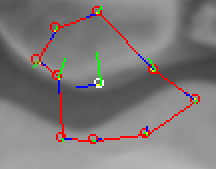
\includegraphics[scale=1.0]{images/ownimpl_forces.png}
    \caption{Darstellung einer aktiven Kontur und deren Kräfte in der umgesetzten Benutzeroberfläche\protect\footnotemark{}}
\label{fig:ownimpl_forces}
\end{figure}
\footnotetext{Eigene Darstellung mittels MATLAB}

Zur Berechnung der \underline{Elastizität eines Punktes} wird das Delta seiner Position zu seinem Nachfolger und Vorgänger addiert und skaliert.
\begin{lstlisting}[caption={Berechnung der Elastizität eines Punktes. Es bedeuten: $p_i$ die Position eines Punktes $i$, $\overline{d}$ die mittlere Seitenlänge zwischen zwei Punkten.\protect\footnotemark}]
    $E_{elas} = (\overline{d} - |p_i - p_{i-1}| )^2$
\end{lstlisting}
\footnotetext{\cite[Seite 147]{hudritsch:script:cp}}

Die \underline{Kurvatur eines Punktes} wird berechnet durch Subtraktion seiner Position von der Summe der Positionen seines Vorgängers und seines Nachfolgers. Seine Position wird mit dem Faktor zwei skaliert.
\begin{lstlisting}[caption={Berechnung der Kurvatur eines Punktes. $p_i$ stellt die Position eines Punktes $i$ dar.\protect\footnotemark}]
    $E_{curv} = |p_{i-1} + p_{i+1} - 2p_i|^2$
\end{lstlisting}
\footnotetext{\cite[Seite 148]{hudritsch:script:cp}}

Die Berechnung der \underline{Energie des Bildes} erfolgt analog derjenigen der Elastizität. Anstelle des Deltas der Position wird das Delta der Farbwerte der unter den Punkten liegenden Pixel genommen.
\begin{lstlisting}[caption={Berechnung der Bildenergie eines Punktes. Es bedeuten: $pv_i$ Farbwert des unter dem Punkt $i$ liegenden Pixels, $\overline{dv}$ mittlere Farbwerte zweier unter den Punkten liegenden Pixel.\protect\footnotemark}]
    $E_{img} = (\overline{dv} - |pv_i - pv_{i-1}| )^2$
\end{lstlisting}
\footnotetext{\cite[Seite 148]{hudritsch:script:cp}}

\newpage

\section{Benutzeroberfläche}
\label{sec:realisation:gui}
Die Applikation verfügt über eine minimal gehaltene Benutzeroberfläche, welche das Laden eines Bildes, das Setzen von Punkten sowie die Definition von kurvenrelevanten Parametern erlaubt. Für die Bildung der aktiven Kontur kann unter den genannten Bildvarianten ausgewählt werden (siehe Abschnitt~\ref{subsec:realization:arch}).

\begin{figure}[h!]
    \centering
    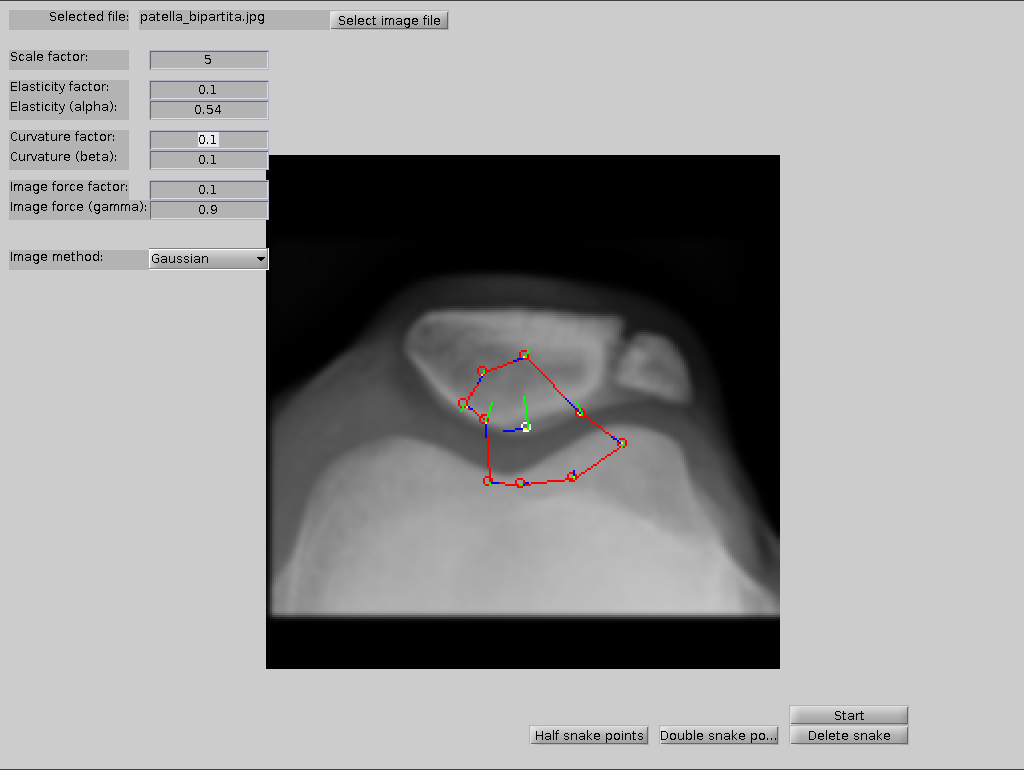
\includegraphics[scale=0.5]{images/ownimpl_gui.png}
    \caption{In MATLAB umgesetzte Benutzeroberfläche\protect\footnotemark{}}
\label{fig:ownimpl_gui}
\end{figure}
\footnotetext{Eigene Darstellung mittels MATLAB}

Kurvenrelevante Parameter sind die folgenden:
\begin{itemize}
    \item \textbf{Ein allgemeiner Skalierungsfaktor}

        Skaliert sämtliche Vektoren in ihrer Darstellung.

    \item \textbf{Elastizität}

        Legt den Einfluss der Elastizität auf die Kurve fest.

    \item \textbf{Kurvatur}

        Legt den Einfluss der Kurvatur auf die Kurve fest.

    \item \textbf{Energie des Bildes}

        Bestimmt den Einfluss der Farbwerte auf die Kurve, aufgrund der Pixel unter den Punkten.
\end{itemize}

\newpage

Die Benutzeroberfläche verfügt über die folgenden Schaltflächen:
\begin{itemize}
    \item \textbf{Start}

        Startet die Bildung der aktiven Kontur.

    \item \textbf{Punkte halbieren}

        Halbiert die Punkte der aktiven Kontur.

    \item \textbf{Punkte verdoppeln}

        Verdoppelt die Punkte der aktiven Kontur.

    \item \textbf{Aktive Kontur löschen}

        Löscht die aktive Kontur mitsamt allen Punkten.
\end{itemize}
